\section{Theorie}
\label{sec:Theorie}

\subsection{Dipole in Ionenkristallen}
Ein Ionenkristall ist eine räumlich periodische Anordnung aus Anionen und Kationen, die durch ionische Bindungen zusammengehalten werden. Bei Caesiumiodid (CsI) sind die Caesiumionen \ce{Cs^+} Kationen, während die Iodidionen \ce{I^+} die Anionen sind.
Durch die Dotierung von solchen Alkalimetallsalzen mit zweiwertigen Kationen wie zum Beispiel Stromtiumionen \ce{Sr^{2+}} können permanente elektrische Dipole erzeugt werden, da der gesamte Kristall ladungsneutral bleiben muss und sich eine Leerstelle bildet. Dies ist in Abbildung \ref{fig:dipolIonenkristall} zu sehen.

\begin{figure}
  \centering
  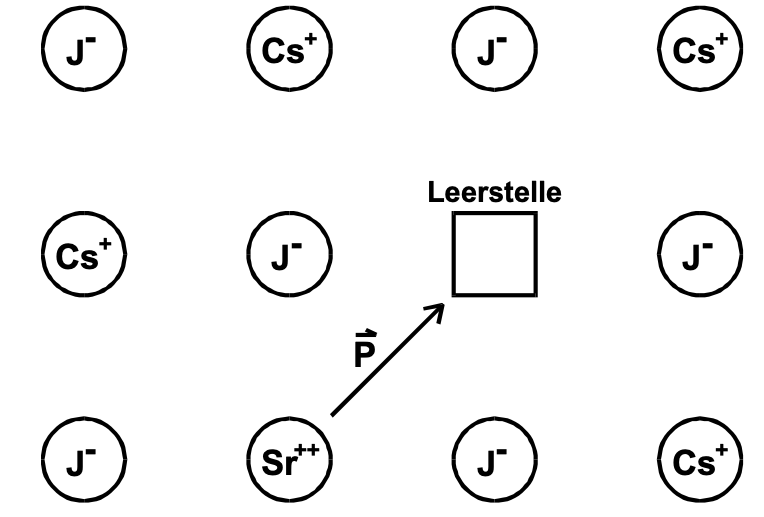
\includegraphics[width=0.8\textwidth]{data/kristall.png}
  \caption{Skizze zur Entstehung eines Dipols in einem Ionenkristall bei Dotierung \cite{anleitungalt}.}
  \label{fig:dipolIonenkristall}
\end{figure}

Es ist auch ersichtlich, dass es nur diskrete Ausrichtungen des Dipols $\vec{P}$ im Festkörper gibt, da dieser vollständig durch die Lage von Leerstelle und Fremdion bestimmt ist. Durch Diffusion der Leerstelle kann der Dipol seine Orientierung ändern. Dazu ist eine materialspezifische Aktivierungsenergie $W$ nötig, da das gitterperiodische Potenzial überwunden werden muss. Die mittlere Zeit zwischen zwei Umorientierungen des Dipols wird Relaxationszeit $\tau$ gennant und beträgt
\begin{equation}
  \tau(T) = \tau_0 \exp\left(\frac{W}{k_{\text{B}}T}\right)
  \label{eqn:relaxtime}
\end{equation}
mit der Temperatur des Kristalls $T$, der Boltzmannkonstante $k_{\text{B}}$ und der charakteristischen Relaxationszeit $\tau_0$.

\subsection{Herleitung des Depolarisationsstroms über die Stromdichte}
Es gibt zwei grundlegende Möglichkeiten, die charakteristischen Größen eines Ionenkristalls $W$ und $\tau_0$ zu bestimmen. Die erste der beiden Möglichkeiten arbeitet mit der Stromdichte $j(T)$, die als Folge der Depolarisation auftritt.

Dazu wird der Ionenkristall in einem elektrischen Feld $E$ betrachtet, sodass sich ein Bruchteil $y$ der Dipole in Richtung des elektrischen Feldes orientiert. Diese Ausrichtung parallel zum Feld konkurriert mit der thermischen Bewegung des Gitters. Es zeigt sich, dass
\begin{equation}
  y(x) = \coth(x) - \frac{1}{x}
  \label{eqn:langevin}
\end{equation}
gilt, wobei $x=(pE)/(k_\text{B}T)$ mit dem Betrag des Dipolmoments $p$.
Dies lässt sich für die in diesem Versuch vorliegenden schwachen elektrischen Felder im Vergleich zur Temperatur zu
\begin{equation}
  y(T) = \frac{pE}{3k_\text{B}T}
  \label{eqn:yApprox}
\end{equation}
nähern.

Dieser Zusammenhang gilt nur, wenn der Ionenkristall ausreichend bei dieser Temperatur verweilt, da die Orientierung der Dipole genauso wie die thermischen Fluktuationen ein statistischer Prozess ist. Wird die Probe bei angelegtem Feld auf eine Temperatur  $T_0$ gekühlt, bei der die Relaxationszeit sehr groß gegenüber den Zeitskalen des Experiments ist, wird ein Einfrieren der Dipole in Feldrichtung beobachtet. Falls nun das äußere Feld ausgeschaltet wird und die Probe mit einer zeitlich konstanten Heizrate $b=\dot{T}$ erwärmt wird, werden die Dipole sich wieder statistisch ausrichten. Dies ruft eine Depolarisationsstromdichte hervor, der sich aus dem Bruchteil der orientierten Dipole bei der Polarisationstemperatur $T_p$ $y(T_p)$, dem Dipolmoment $p$ und der Relaxationsrate pro Volumen $\frac{\symup{d}N}{\symup{d}t}$ zusammensetzt:
\begin{equation}
  j(T) = y(T_p) p \frac{\symup{d}N}{\symup{d}t}\,.
  \label{eqn:jAnsatz}
\end{equation}
Für den ersten Term lässt sich der Ausdruck aus Gleichung \eqref{eqn:yApprox} einsetzen und für $N$ lässt sich eine Relaxationsgleichung mit der Relaxationszeit $\tau(T)$ ansetzen, sodass sich unter Verwendung von \eqref{eqn:relaxtime}
\begin{equation}
  j(T) = \frac{p^2 E}{3 k_\text{B} T_p} {N_p}{\tau_0}
         \exp \left(- \frac{1}{b \tau_0} \int_{T_0}^{T} \exp(-W/(k_\text{B}T') \symup{d}T' \right) \exp\left(\frac{W}{k_{\text{B}}T}\right)\,.
  \label{eqn:depolKurve}
\end{equation}
ergibt. Der Kurvenverlauf von $j(T)$ ist bereits aus allgemeinen Überlegungen ersichtlich: Für tiefe Temperaturen wird der Depolarisationsstrom steil bis zu einem Maximum ansteigen, da die Relaxationszeit schnell mit der Temperatur abnimmt, um danach wieder exponentiell zu sinken, weil die Anzahl der noch nicht relaxierten Dipole immer weiter abnimmt. Ein zweites Maximum, das zu einer höheren Aktivierungsenergie gehört, kann möglicherweise im Experiment für noch höhere Temperaturen beobachtet werden. Ein typischer
Kurvenverlauf ist in Abbildung \ref{fig:kurve} zu sehen.

\begin{figure}
  \centering
  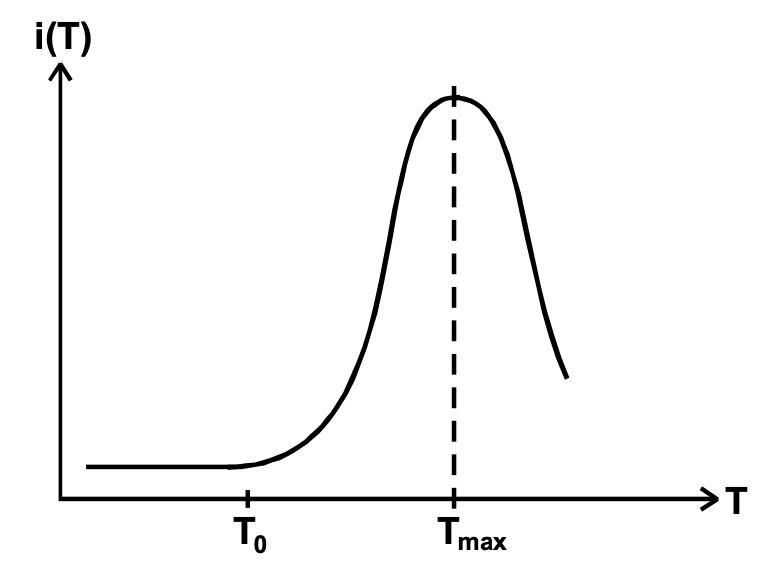
\includegraphics[width=0.8\textwidth]{data/kurve.png}
  \caption{Typischer Kurvenverlauf für den Depolarisationsstrom in Abhängigkeit von der Temperatur \cite{anleitungalt}.}
  \label{fig:kurve}
\end{figure}

Für den Anfang dieses Verlaufs bei niedrigen Temperaturen ist das Integral in der Exponentialfunktion näherungsweise null, sodass die Depolarisationskurve im Anfangsbereich zu
\begin{equation}
  j(T) \approx \frac{p^2 E}{3 k_\text{B} T_p} {N_p}{\tau_0}
               \exp\left(\frac{W}{k_{\text{B}}T}\right)
               \label{eqn:naeherung}
\end{equation}
genähert werden kann. Es ist dann möglich, in diesem Bereich eine Ausgleichsrechnung $\ln j$ gegen $\frac{1}{T}$ durchzuführen, um $W$ zu ermitteln.

\subsection{Herleitung des Depolarisationsstroms über den Polarisationsansatz}

Es ist auch möglich, die Aktivierungsenergie und die charakteristische Relaxationszeit über den gesamten Kurvenverlauf zu ermitteln. Dazu wird betrachtet, dass die Änderung der Polarisation der Probe einen Strom hervorruft.
Es zeigt sich, dass mit dem Strom $i(T)$ der Zusammenhang
\begin{equation}
  \frac{W}{k_\text{B}T} = \ln \frac{\int_T^\infty i(T')\,\symup{d}T'}{i(T) \tau_0 b}
\end{equation}
gilt, sodass bei Kenntnis des Stromverlaufs $i(T)$ eine Ausgleichsrechnung erfolgen kann, um $W$ und gegebenenfalls auch $\tau_0$ zu bestimmen.
Eine andere Möglichkeit besteht darin, $\tau_0$ aus dem Maximum der Depolarisationskurve zu bestimmen. Dafür gilt
\begin{equation}
  \tau_0 = \frac{k_\text{B}T_{\text{max}}^2}{Wb}\exp\left(-\frac{W}{k_\text{B}T_\text{max}}\right)
\end{equation}
mit der Lage des Strommaximums $T_\text{max}$.
